\chapter{The ATLAS Trigger System}
\label{ch:trigger}

	The ATLAS trigger system together with its performance will be presented in this chapter. A brief introduction, about the reason behind the need of a trigger system together with its implementation in ATLAS will be discussed in Section~\ref{sec:Trig_intro}. The algorithms used for the tracking in the inner detector will then be described in Section~\ref{sec:tracking}. Ultimately, measurements of the performance of the low transverse momentum single lepton triggers and medium and high trasnverse momentum \bj\ triggers, as part of the \textit{qualification task}\footnote{In order to become an ATLAS author, a person must have been an active ATLAS member for at least one year working on a technical work} of the author, will be discussed in Section~\ref{sec:Trig_perf}. 



	\section{Overview}
	\label{sec:Trig_intro}

		More than 80 \ifb\ of \pp\ collisions were delivered in 2016 and 2017 by the LHC. As previously mentioned in Section~\ref{sec:trigSyst}, due to storage space limitations it is not feasible to save all the information about the collision after every bunch crossing, so the ATLAS Trigger System is indispensable to reduce the read-out rate to a sensible value without affecting the physics programme of ATLAS, \eg\ discarding potentially interesting events. A multiple-level architecture is employed to allow the trigger some more time such that the identification, of an interesting event, using both software- and hardware-based real-time algorithms to determine whether or not a bunch-crossing contains interesting physics, is made possible. 

		\begin{figure}[!htb]
			\centering
			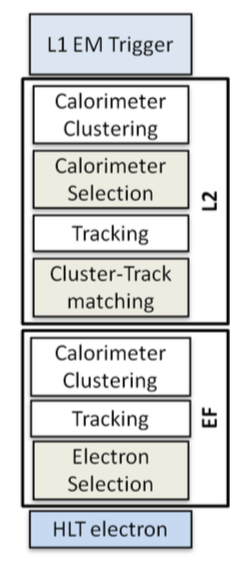
\includegraphics[height=.3\textheight]{Trigger/trig_chain}
			\caption{\label{fig:trig_chain} An Electron-trigger chain (from \cite{ATLASTrigger2010}).}
		\end{figure}

		The trigger system is configured via the so-called trigger \textit{menu} that is meant to define the trigger \textit{chains} - usually referred to just as trigger - that start from a L1 trigger and specify a sequence of reconstruction and selection steps for the specific trigger signatures required in the trigger chain. Fig.~\ref{fig:trig_chain} shows an illustration of an electron-trigger chain used to select electrons \cite{ATLASTrigger2010}.

		The two levels will be discussed in the following sections.


		
		\subsection{Level 1 Trigger}
		\label{sec:L1}

			The Level 1 (L1) trigger decision is formed by the Central Trigger Processor (CTP), based on information from the calorimeter trigger towers and dedicated triggering layers in the muon system. The CTP forms the L1 trigger decision by applying the multiplicity requirements and prescale factors specified in the trigger menu to the inputs from the L1 trigger systems. The CTP also provides random triggers and can apply specific LHC bunch crossing requirements. The L1 trigger decision is distributed, together with timing and control sig- nals, to all ATLAS sub-detector readout systems.

			The first level, known as Level 1 (L1) trigger, is a hardware-based stage. It processes low-granularity information from the calorimeter and the muon spectrometer and identifies the so-called Regions of Interest (RoIs)\footnote{$\eta - \phi$ regions where event features have been found by the L1 selection process.} before making a decision. It then feeds the next level, the high-level trigger (HLT) which will perform further investigations. L1 is implemented in fast custom electronics to keep the decision time around 2.5 $\mu$s. Event data from other sub-sytstem are temporarily stored in memories whilst L1 decision is taken. 			

			During the long shutdown (LS1), various upgraded were implemented in order to prepare for the expected higher rates in Run 2. A new topological trigger (L1-Topo) consisting of two FPGA-based (Field-Programmable Gate Arrays) processor modules was added in L1. L1-Topo~\cite{ATLASL1Topo} is fed with energy and direction information, about the objects found by the L1 calorimeter and the muon trigger, which will be processed by dedicated algorithms implemented in its own FPGAs. However, due to the 100 kHz read-out rate, not all the information collected by L1-Topo will be sent to the HLT. In order to properly seed the RoI-guided HLT reconstruction, speficic objects in combination with the correct topological criteria must be employed.




		\subsection{High-Level Trigger}
		\label{sec:HLT}

		%BEN's

		% The rest of the trigger is made up of software running on a commercially available computer cluster and is known as the high level trigger (HLT). In Run 1 the HLT was split into two levels: the level 2 (L2) and event filter (EF) triggers. The L2 was custom written software which processed data at the full detector granularity within the RoIs from L1. It performed calorimeter reconstruction, the earliest available Fast Tracking, and track-cluster matching. It had a peak output of about 6.5 kHz with an average decision time of about 75 ms. The EF was an optimised version of the standard ATLAS reconstruction software which can run on the full granularity data from the entire detector. It performed the full reconstruction and precision tracking to make the final event selection. It had a peak output rate of about 700 Hz with an average decision time of about 1 s. Each of these stages ran separately with a new node in the computer cluster being assigned to the event between the L2 accepting the event and the event filter making a decision on the event.

		% In Run 2 the HLT has been merged into a single process running on a single HLT computing cluster node. This simplifies the data-flow removing the need for network communication between the L2 and EF triggers and removes the duplication in requesting data from the DAQ system. It also means the EF trigger doesn’t have to first perform event building after the L2 accept as the event building can flexibly be placed as a step during the processing of the algorithms on the single HLT CPU node. The new combined trigger has a peak output rate of about 1 kHz and an average decision time of about 200 ms. A new hardware-based track preprocessor known as the Fast TracKer (FTK) [35] is planned to be added in Run 2. It will process events after the L1 trigger accept in order to seed the HLT algorithms.


			The HLT is used to reduce the output rate down to 1 kHz and it has a $\sim$200 ms average decision time. Events that pass L1 trigger are then processed by the HLT using finer-granularity calorimeter information, precision measurements from the MS and tracking information from the ID. The HLT reconstruction can be run within RoIs identified at L1 or a so-called full-scan on the full detector can be performed. The track reconstruction in the Inner Detector is an essential component of the trigger decision in the HLT and it will be discussed more in detail in Chapter~\ref{ch:trigger}




	\section{The tracking}
	\label{sec:tracking}



	\section{Performance of HLT}
	\label{sec:Trig_perf}

		\subsection{Electrons}

		\subsection{Muons}

		\subsection{$b$-jets}

